\documentclass{article}
\usepackage[francais]{babel}
\usepackage[UTF8]{inputenc}
\usepackage[T1]{fontenc}
\usepackage{graphicx}
\usepackage{fancyhdr}
\usepackage{eurosym}
\usepackage{color}
\usepackage{soul}

\pagestyle{fancyplain} \chead{}\lhead{\textit{Les Professionnels}} \rhead{\emph{\textit{Evasion}}}

\definecolor{pseudorouge}{RGB}{200, 50, 50}
\definecolor{pseudoblue}{RGB}{20,10,230}
\definecolor{texteGris}{RGB}{50,50,75}

\begin{document}
\thispagestyle{empty}
\begin{center}
\fontsize{21}{21}{\textbf{Rapport de Soutenance 2 \vspace*{0.2cm}\newline\textit{Evasion}}}
\end{center}

\vspace*{0.7cm}

\begin{center}
\fontsize{21}{21}{\textbf{- Les Professionnels/}}
\fontsize{21}{21}{\textbf{2013-2014 -}}
\end{center}

\vspace*{0.5cm}

\begin{center}
\includegraphics[scale=01.0]{evasion}
\end{center}

\vspace*{0.5cm}

\fontsize{14}{14}
\begin{center}
{Lenny \textcolor{pseudorouge}{\textit{"Le Noob"}} Danino - danino\_l}
\end{center}
\begin{center}
Louis \textcolor{pseudoblue}{\textit{"El Parain"}} Kédémos - kedemo\_l
\end{center}
\begin{center}
Anatole \textcolor{pseudoblue}{\textit{"Totonut"}} Moreau - moreau\_a
\end{center}
\begin{center}
Khalis Chalabi - chalab\_k
\end{center}

\begin{center}
\includegraphics[scale=00.20]{infini}
\end{center}

\newpage
\thispagestyle{empty}
\pagestyle{fancyplain} \chead{}\lhead{\textit{Les Professionnels}} \rhead{\emph{\textit{Evasion}}}
\tableofcontents



\newpage
\fontsize{12}{12}
\pagenumbering{arabic}
\section{Introduction}
\par
Plus de deux mois se sont écoulés depuis la 1ère soutenance et on peut dire qu’on a bien progressé !
Durant cette période nous avons d’abord pris un laps de temps de repos mais qui permis de mieux nous reconcentrer pour la suite.
De ce fait nous avons terminé une partie des tâches qui nous incombées de faire pour cette soutenance depuis la première et puisque nous aimons déjà notre jeu nous avons fait en sorte de le rendre vraiment beau !
\newline
\par
Par rapport à nos prévisions il va de soi qu’elles ont été respectées malgré nos épreuves importantes qui ont marqué nos emplois du temps.
Actuellement notre jeu est déjà à un stade intéressant puisque dorénavant on peut avoir un bon aperçu des décors, des personnages, du multijoueur…
\newline
\par
Aujourd’hui notre groupe est plus que soudé, tant par le temps que nous avons passé ensemble  que par  l'importance que nous éprouvons tous pour ce projet. Cela s’est fait en partageant nos désirs, problèmes rencontrés et idées. Plusieurs fois nous avons décidé de se retrouver pour parler et programmer ensemble, de manière plus efficace. 
\newline
\par
Notre précédente note nous a encouragés à donner le meilleur de nous-mêmes, pour avoir une identique et même plus ! Ce projet est donc devenu un véritable engouement pour chacun et c’est toujours avec plaisir que nous nous retrouvons, à la différence d’un simple groupe qui n’accorderais aucune ou peu d’importance à ce projet.
\newline
\par
Nous avons écouté les remarques faites lors de la première soutenance et avons tout fait pour que cette fois, le jeu vous plaise encore plus. Notre site a été refait et certains d’entre nous se sont concentrés davantage sur le code pour rendre le jeu réellement fonctionnel.
\newline
\par
Malgré cela, la soutenance n'en reste pas moins un certain défi, que nous espérons relever pour continuer sur notre lancée.
Ce rapport détaillera donc les nouvelles caractéristiques du jeu et présentera également les prévisions pour la soutenance suivante.
\newpage

\section{Avancements}
\subsection{Louis\textcolor{pseudoblue}{\textit{"El Parrain"}} Kedemos}

\subsubsection{Expérience personnelle}
Avant cette soutenance, nous avons disposé de deux semaines de vacances, ou du moins, de deux semaines sans cours. Je pense que cela a été bénéfique pour réaliser une grosse avancée dans notre projet. En effet, nous n'avons pas eu cette fois-ci le stress lié aux révisions ou aux cours. Se réunir pendant ces deux semaines a été plus facile qu'en période de cours. \newline
Comme à la première soutenance, j'ai dû laisser de côté certaines idées de réalisations. J'espère avoir le temps, pour la troisième soutenance, de les réaliser. En revanche, certaines choses, que je n'avais pas prévu à l'origine, ont été développées.

\subsubsection{Avancement de la 3D}
Notre jeu est développé en \bsc{3D}. Mettre de côté ce point pendant le développement du jeu est impensable. C'est pourquoi de gros progrès ont été réalisés à ce niveau. Au moment de la première soutenance, pour créer un personnage ou un mur en \bsc{3D}, il fallait faire tout un tas de déclarations dans le fichier du jeu principal. Il devenait urgent de rendre la création \bsc{3D} plus facile, pour permettre des phases de tests le plus tôt possible. J'ai donc écrit des classes qui rendent possible l'instanciation, l'affichage et la manipulation des modèles \bsc{3D} aisés :

\begin{quote}
\textcolor{texteGris}{
Evasion.Affichage.\_3D.Perso\_Model michael;\\
michael = new Affichage.\_3D.Perso\_Model(Content, new Vector3(20, 0, 20), viewMatrix, aspectRatio, graphics, 1);\\
michael.Update();\\
michael.Draw();}
\end{quote}

Ces quatre lignes, placées au bon endroit, nous permettent de manipuler un personnage en \bsc{3D}. On peut le faire se déplacer dans les quatre directions, on peut le faire tourner sur lui même.\\

Les déplacements ont été l'un des principaux problèmes que j'ai rencontré. Pour modifier la position ou la rotation d'un modèle dans son espace \bsc{3D}, l'utilisation de matrices est nécessaire. Il faut effectuer plusieurs produits matriciels à la suite. En premier, on multiplie la matrice de position du squelette du modèle par l'échelle souhaitée. Cela permet un redimensionnement. On multiplie ensuite le résultat par trois matrices de rotation, une pour chaque axe. Enfin, on multiplie le résultat par la translation que l'on souhaite faire faire au modèle. Tout cela permet d'obtenir une bonne rotation et une bonne translation du modèle \bsc{3D}. 
Or, le produit matriciel n'est pas commutatif. C'est à dire que pour deux matrices A et B, le produit \bsc{AB} est différent du produit \bsc{BA}. Pour la première soutenance, je n'avais pas suivi le même ordre que celui énoncé précédemment. Le résultat obtenu n'était donc pas celui espéré. Les cours de math qui ont suivi la première soutenance portaient sur les matrices. J'ai ainsi pu me rendre compte de mon erreur. La première illustration montre comment le personnage se déplaçait lors de la première soutenance : 

\begin{figure}[h]
\begin{center}
\includegraphics[scale=0.5]{deplac1.jpg}
\caption{Déplacement première soutenance}
\end{center}
\end{figure}
On peut voir que le personnage ne pouvait que se rapprocher ou s'éloigner du centre et tourner par rapport au centre. Régler le problème des matrices a permis de rendre le déplacement plus naturel. Le personnage peut maintenant se déplacer dans quatre directions et tourner sur lui-même. La seconde figure illustre ces déplacements : 

\begin{figure}[h]
\begin{center}
\includegraphics[scale=0.5]{deplac2.jpg} 
\caption{Déplacement deuxième soutenance}
\end{center}
\end{figure}

\subsubsection{Travail sur les collisions}
Après avoir régler l'affichage et le déplacement des modèles, il a fallut s'occuper des collisions. Dans le monde du jeu vidéo, les collisions sont ce qu'il y a de plus important. Si les collisions sont mal gérées, lors d'un combat par exmple, l'ennemi peut nous frapper mais pas le contraire. \\
Je suis allé cherché des informations concernant les collisions sur internet. Les résultats ne manquaient pas. De nombreuses techniques sont expliquées. Il y a par exemple celle utilisant des \bsc{BoundingBox}. Des coordonnées définissent une boîte en trois dimensions contenant le modèle. Ensuite une méthode permet de savoir si deux \bsc{BoundingBox} sont en collisions. Une autre méthode consiste à utiliser les coordonnées d'un modèle et à regarder où il se situe par rapport aux autres modèles. Si deux coordonnées sont trop proches, alors on estime qu'il y a collision.\\
Nous avons choisi de retenir la méthode utilisant les \bsc{BoundingBox}. Elle permet de tester les collisions de manière souple et rapide. Voici une illustration qui montre comment sont gérés les \bsc{BoundingBox} par XNA : 

\begin{figure}[h]
\begin{center}
\includegraphics[scale=0.7]{BoundingBox.jpg}
\caption{Gestion des \bsc{BoundingBox}}
\end{center}
\end{figure}

Les traits blanc représentent les \bsc{BoundingBoxes}. L'utilisation de celles-ci est pratique surtout lorsque le personnage tourne. Les \bsc{BoundingBoxes} sont aussi tournées de la même manière que le personnage. Ainsi, il n'y a pas besoin de faire de calcul pour trouver les nouvelles coordonnées des \bsc{BoundingBoxes}. Les coordonnées sont mises à jour automatiquement. \\
Une autre solution serait d'utiliser des \bsc{BoundingSpheres}. C'est le même principe que les \bsc{BoundingBoxes}, mais avec des spheres. Cette solution est la plus simple parmi celles que j'ai pu trouver. Mais elle ne permet pas de faire de détection de collisions précises avec les murs, qui eux, sont plats.

\subsubsection{Ce qu'il reste à faire}

Bien que nous ayons bien avancés, il reste un certain travail à faire. Le système de collision sera grandement amélioré, pour être plus rapide et plus précis. Je m'occuperai aussi de rajouter les animations des personnages. Dans le deuxième rendu du projet, ils restent statiques. Cela peut paraître un peu bizarre lorsque l'on joue à un jeu. Enfin il reste la plus grande partie de la logique du jeu à implémenter, telle que la gestion des objectifs de la partie, le déplacement des ennemis...

\newpage

\subsection{Khalis Chalabi}

\subsubsection{Avancement du projet}

\par
Dans cette partie je vais vous présenter dans un premier les différentes tâches que j'ai accomplies pour cette deuxième  soutenance et les problèmes que j'ai rencontrés.
\newline
\newline
\underline{Finalisation des classes Personnages, Objets et Décors :}
\newline

\par
Lors de la première soutenance Lenny et moi avons implémenté les classes mères Personnages, Objet et Décors mais il manquait quelques classes filles. Pour cette soutenance je me suis donc occupé des classes filles PNJ (personnages non jouables), objets utilitaires et outils avec l’aide de Lenny. Ces classes n’ont pas été très difficiles à implémenter car elles héritaient des classes mères. Elles n’avaient besoin que de constructeurs et éventuellement de quelques propriétés ou méthodes supplémentaires. Je pense qu’au cours de l’avancement du projet il y aura peut-être quelques modifications à ajouter à ces classes en fonction des bugs et de nos envies personnelles mais elles sont globalement finies.
\newline
\newline
\underline{Texture de personnages et des murs :}
\newline

\par
Cette tâche fût une des plus difficiles à réaliser car il fallait que j’utilise deux logiciels avec lesquels je n’avais jamais travaillé :\bsc{ Photoshop} et\bsc{ Blender}. Nous faisons un jeu en \bsc{3D} donc il ne suffit pas d’importer des sprites et des textures avec \bsc{XNA} comme pour un jeu en \bsc{2D}. Louis a créé ce qu’on appelle des modèles avec l’aide du logiciel \bsc{Blender}. Ce logiciel permet, entre autre, de modéliser des images en \bsc{3D}. Nous avions donc la forme principale de nos personnage, il fallait ensuite les personnaliser (lui faire porter des vêtements, lui faire un visage…) Il nous a d’abord fallu découper notre modèle pour obtenir un patron car pour personnaliser le personnage il faut appliquer une texture sur chacune des faces du modèle.
\newline

\begin{figure}[t]
\begin{center}
\includegraphics[scale=0.3]{decoupe.jpg}
\caption{Patron du personnage}
\end{center}
\end{figure}

\newpage

\par
Pour découper notre modèle nous avons utilisé \bsc{Blender}, il fallait découper les faces mais en faisant attention d’en garder une qui soit rattacher aux autres. Imaginer la découpe d’un cube nous a beaucoup aidé. Une fois le modèle complètement découpe nous obtenons l’image ci-dessus.         
Vous avez peut-être l’impression que cela ne ressemble à rien mais en reconstruisant le patron vous obtenez bien le modèle de notre personnage. En haut à gauche de l’image vous avez ses deux bras, juste en dessous et sur la droite ses deux jambes, la plus grosse figure correspond au haut du corps (torse, dos, cou…) et enfin tout en bas à droite sa tête.

\par
Une fois ce travaille fait il fallait donner l’aspect que nous voulions au personnage. Pour cela j’ai dû utiliser le logiciel \bsc{Photoshop} car pour chaque face du patron il faut comme je vous l’ai dit précédemment une texture. Je me suis occupé de faire le personnage principal ainsi que les gardiens de prison. Je sélectionnais une image qui me plaisait sur Internet puis je prenais la partie qui m’intéressait grâce aux fonctionnalités de \bsc{Photoshop}. Par exemple pour faire le dos du gardien j’ai choisi une image de gardien de prison vu de dos puis j’ai rogné l’image de façon à avoir que le haut de l’uniforme. La difficulté dans cette partie était que je n’avais jamais utilisé \bsc{Photoshop} donc j’ai dû  découvrir ce logiciel au fur et à mesure. Lorsque j’avais des problèmes je me renseignais sur Internet ou demandais de l’aide à Louis qui connait plutôt bien ce logiciel. M’occuper du design des personnages m’a donc demandé beaucoup de temps. Je devais faire de nombreux tests pour obtenir ce que je voulais.    
\newline

\begin{figure}[htbp]
\begin{minipage}[c]{.45\linewidth}
\begin{center}
\includegraphics[scale=2]{michaelphotoshop.png}
\caption{Texture personnage principal}
\label{fig:michaelphotoshop}
\end{center}
\end{minipage}
\hfill
\begin{minipage}[c]{.45\linewidth}
\begin{center}
\includegraphics[scale=2]{bellikphotoshop.png}
\caption{Texture gardien de prison}
\label{fig:bellikphotoshop}
\end{center}
\end{minipage}
\end{figure}

\par
Une fois que j’avais fini d’appliquer des textures au patron, j’importais l’image sur \bsc{Blender} pour pouvoir voir l’aspect de mon personnage parce qu’avec le patron, comme vous pouvez le voir, on ne s’en rend pas compte. Je regardais l’aspect de mon personnage à chaque modification pour pouvoir éviter de tout recommencer si ça ne me plaisait pas.
\newline

\newpage
\begin{figure}[htbp]
\begin{minipage}[c]{.45\linewidth}
\begin{center}
\includegraphics[scale=0.6]{michael.png}
\caption{Personnage principal}
\label{fig:michael}
\end{center}
\end{minipage}
\hfill
\begin{minipage}[c]{.45\linewidth}
\begin{center}
\includegraphics[scale=0.5]{bellik.png}
\caption{Gardien de prison}
\label{fig:bellik}
\end{center}
\end{minipage}
\end{figure}

\par
Une fois le premier personnage fait le deuxième fût plus simple à faire car j’avais pu m’habituer à \bsc{Photoshop} et à \bsc{Blender}. Le plus facile dans cette partie fût la réalisation du mur de la prison. Etant donné qu’en \bsc{3D} un mur est juste un rectangle le découpage est plutôt simple par rapport au découpage du modèle du personnage. Il suffisait ensuite d’importer l’image d’un mur dans \bsc{Photoshop} puis de légèrement la modifier.
\newline
Cela nous a donc permis d’avoir les principaux personnages et le début du décor.
\newline

\underline{Implémentation de la barre de vie :}
\newline

\par
Comme dans la plupart des jeux vidéo, notre personnage possède une barre de vie. Cette dernière se vide en fonction des dégâts reçus et peut se remplir si le personnage se soigne. Elle possède en son centre un nombre qui permet de connaitre le nombre de point de vie actuel sur le nombre de point de vie maximum. Pour créer cette barre de vie j’ai implémenté une nouvelle classe nommée ‘’BarreDeVie’’.

\par
Avant de commencer à coder, j’ai tout d’abord créé le design de ma barre de vie à l’aide de \bsc{Photoshop}. J’ai dû créer deux textures : la barre de vie et sa bordure. Une fois cette étape réalisée j’ai pu commencer à implémenter ma classe. Ce ne fut pas très long, la classe ne contenait qu’un constructeur et 4 fonctions. La première fonction me permettait d’ajuster la barre de vie de telle sorte que les points de vie ne soit pas négatif ou qu’il  ne dépasse pas la valeur maximale définie. Ensuite une fonction qui mettait à jour la barre de vie par rapport au niveau de sante du personnage. Puis pour finir les deux fonctions les plus difficiles. Celle qui permet de réduire la barre de vie normalement et celle qui la dessine dans les bonnes proportions. En effet, lorsque les points de vie diminuait ou augmentait la totalité de la barre (le fond rouge ainsi que la bordure) diminuait également mais se rapetissait jusqu’à devenir extrêmement fine et minuscule ! De plus elle se dessinait dans de mauvaises proportions car elle  prenait toute la longueur de l’écran. Pour régler ces problèmes j’ai utilisé deux surcharges différentes de la fonction ‘’Draw’’ une pour la bordure et l’autre pour le fond. Pour que la vie diminue correctement j’ai juste fait un peu de maths ! L’affichage du nombre de point de vie est tout simplement l’utilisation d’un ‘’SpriteFont’’. Pour que tout s’affiche correctement il ne manquait plus qu’à déclarer, initialiser, charger et dessiner la barre de vie dans la classe ‘’game’’.

\begin{figure}[h]
\begin{center}
\includegraphics[scale=1.5]{Barredevie.png}
\caption{Barre de vie}
\end{center}
\end{figure}

\underline{Le mode Multijoueur :}
\newline

\par
Un de mes objectifs pour cette deuxième soutenance était de commencer à implémenter un mode multijoueur. Je pense que je m’en suis plutôt bien sorti car il est pratiquement fini (on peut donc dire que je suis légèrement en avance sur cette partie la). Je ne savais pas par où commencer, j’ai dû faire quelques recherches pour comprendre comment débuter. Je voulais faire un mode multijoueur avec un écran scindé où les joueurs verrait chacun leur personnage. J’ai donc suivi un tutoriel sur \bsc{Youtube} qui expliquait comment scindé un écran en deux. Il y a une classe nommée ‘’Viewport’’ qui facilite justement la division de l’écran. Il suffit juste ensuite de copier ce qui se trouve dans l’écran de gauche dans celui de droite. Bien sur le tutoriel était pour un jeu en \bsc{2D} du coup il m’a fallu tester et modifier certaines choses pour que cela fonctionne
\newline
Pour que la séparation soit nette, j’ai créé une texture avec \bsc{Photoshop} que j’ai ensuite importé avec \bsc{XNA}. Il est donc plus facile de distinguer les deux ‘’écrans’’. 
\newpage
\begin{figure}[h]
\begin{center}
\includegraphics[scale=1]{Multijoueur.png}
\caption{Mode multijoueur}
\end{center}
\end{figure}

\par
Chaque joueur a son propre personnage, sa propre barre de vie ainsi que sa propre camera. L’essentiel du mode multijoueur est donc fait, il ne manquera plus qu’à l’améliorer. Pour finir, j’ai créé un bouton multijoueur en plus dans le menu d’accueil ce qui permet de jouer le mode solo ou le mode multijoueur.
\newline

\underline{Le site web :}
\newline

\par
Nous avions déjà un site lors de la première soutenance, mais pour celle-ci nous avons décidé de modifier le design du site ainsi que la clarté du code. C'était à Anatole et moi même de nous occuper de cette tâche. J'ai, avant tout, refait le design du site en faisant un croquis sur une feuille de papier. J'ai dû  ensuite me replonger dans un tutoriel du site du Zero portant sur les bases du langage web : \bsc{HTML5} et le \bsc{CSS3}. J'ai donc participé à la mise en place du site de notre jeu vidéo en faisant du \bsc{HTML}, du \bsc{CSS} et, enfin, en faisant son design.
\newline

\newpage
\underline{Problèmes rencontrés :}
\newline

\par
Pour cette deuxième soutenance j’ai dû découvrir de nombreuses choses pour pouvoir avancer dans les parties qui m’étaient confiées. Je ne savais pas utiliser les logiciels \bsc{Photoshop} et \bsc{Blender} et je ne savais pas comment implémenter le mode multijoueur. Il a donc fallu que je fasse des recherches de mon côté pour pouvoir produire quelque chose. C’est cette partie qui fut je pense la plus compliquée car je ne savais jamais si ce que j’avais trouvé aller convenir à notre projet. Je devais faire donc des tests et puis si cela ne fonctionnais pas faire de nouvelles recherches. Cependant, je trouvais généralement tout ce que je voulais sur Internet et si je ne trouvais pas je pouvais quand même demander à Louis ou Anatole. 

\par
Le mode multijoueur fut la tâche la plus difficile à accomplir pour cette deuxième soutenance, spécialement le passage en plein en plein écran. Le mode multijoueur ne s’adaptait pas au plein écran et la barre de séparation disparaissait. Pour cette partie-là j’ai dû demander l’aide d’Anatole car il avait eu affaire au même problème pour le menu. Une des surcharge de la fonction ‘’Draw’’ et des modifications sur l’utilisation de la classe ‘’Viewport’’ nous permis de résoudre le problème.

\par
Malgré ces problèmes je peux quand même constater que je progresse car j’ai pu effectuer de nombreuses tâches pour cette deuxième soutenance que j’aurais été incapable de réaliser auparavant.
\newline
  
\subsubsection{Et après ?}

Pour la troisième soutenance je vais me fixer plusieurs objectifs à atteindre :
\newline

\underline{Finalisation du mode multijoueur :}
\newline
\par
Je vais continuer mon travail sur le multijoueur en l'améliorant. J’aimerais pouvoir ajouter un ‘’timer’’ qui permettrait de déclarer vainqueur le premier joueur qui aurait réussi à sortir de la prison.  
\newline

\underline{Le mode réseau :}
\newline
\par
Je vais tenter de participer a l'implémentation du mode réseau. Cette partie m'a l'air plutôt difficile. Je ne pense pas que nous ferons plus que mettre le score obtenus lors d'une partie.
\newline

\underline{Les graphismes :}
\newline
\par
Aucun objet apparait encore dans le jeu car nous n'avons pas fait leur graphisme, je vais donc m'en occuper pour cette troisième soutenance. Je pense aussi participer au graphisme correspondant au décor. Je sais plutôt bien utiliser \bsc{Photoshop} maintenant donc je pense que mon aide sera très utile. Nous aurons donc une vraie prison pour la troisième soutenance.  
\newline

\underline{Le site web :}
\newline
\par
Je pense qu'il faudra améliorer le site web, je vais donc m'en occuper avec Anatole. Nous avons eu l'idée, par exemple, de faire un onglet ''Langues'' qui permettra à l'utilisateur de mettre le site en français ou en anglais.    

\newpage

\subsection{Lenny \textcolor{red}{"Le Noob"} Danino}
\subsubsection{Personnages/Décors}

\par
Les textures des personnages sont des éléments très important dans le jeu car elles sont ce qui est immédiatement regardées par les joueurs. Il faut qu’elles soient jolies et agréables sinon les joueurs ne voudront pas jouer au jeu. Ainsi nous avons décidé qu’il serait préférable de dessiner par-dessus des textures provenant d’images sur internet. Cela apporte un degré de réalisme non négligeable.
\newline
\newline
\underline{Réalisations:}

\par
\underline{Les textures et le code:}
\newline

\par
Premièrement il a fallu réaliser un modèle de base pour les personnages découpés avec Blender.  Ce logiciel est extrêmement utile mais je n’y avais jamais touché et il m’a donc fallu l’aide de Louis et de tutoriels pour parvenir à me débrouiller suffisamment. Nous avons préféré rendre notre personnage cubique. C’était intéressant à faire car cela nécessitait de visualiser l’ensemble dans l’espace comme lorsqu’on découpe un cube.

\begin{figure}[h]
\begin{center}
\includegraphics[scale=0.25]{decoupe.jpg}
\caption{Decoupe d'un personnage}
\end{center}
\end{figure}

\newpage
En me basant sur le modèle j’ai pu créer les textures de 2 personnages. J’ai utilisé Photoshop, qui comme Blender m’était entièrement inconnu, pour la correction des images et la découpe. Puis j’ai visualisé le résultat avec Blender. Je vous présente donc le Pnj des prisonniers :
\newline


\begin{figure}[htbp]
\begin{minipage}[c]{.45\linewidth}
\begin{center}
\includegraphics[scale=0.5]{prisonnierblend.png}
\caption{Prisonnier}
\end{center}
\end{minipage}
\hfill
\begin{minipage}[c]{.45\linewidth}
\begin{center}
\includegraphics[scale=0.2]{prisonnier.png}
\caption{Texture prisonnier}
\end{center}
\end{minipage}
\end{figure}


Et voici un des ennemis en dehors de la prison : 
\begin{figure}[h]
\begin{center}
\includegraphics[scale=0.4]{ennemidehorsblend.png}
\caption{Ennemi extérieur}
\end{center}
\end{figure}

\begin{figure}[h]
\begin{center}
\includegraphics[scale=0.3]{ennemidehors.png}
\caption{Texture ennemi extérieur}
\end{center}
\end{figure}


\newpage

\par
Cependant dessiner des personnages reste un aspect graphique. J’ai dû en effet toucher au code des classes pour pouvoir les insérer. Avec l’aide de Khalis, qui s’est occupé d’autres personnages, j’ai donc terminé les classes Pnj, Objets Utilitaires et Outils.
De même je m’étais occupé dans la première soutenance des classes Décors, Murs et Objets. Pour parfaitement les terminer j’ai dû effectuer les mêmes étapes que pour les personnages.
\newpage
Voici le modèle des murs :
\begin{figure}[h]
\begin{center}
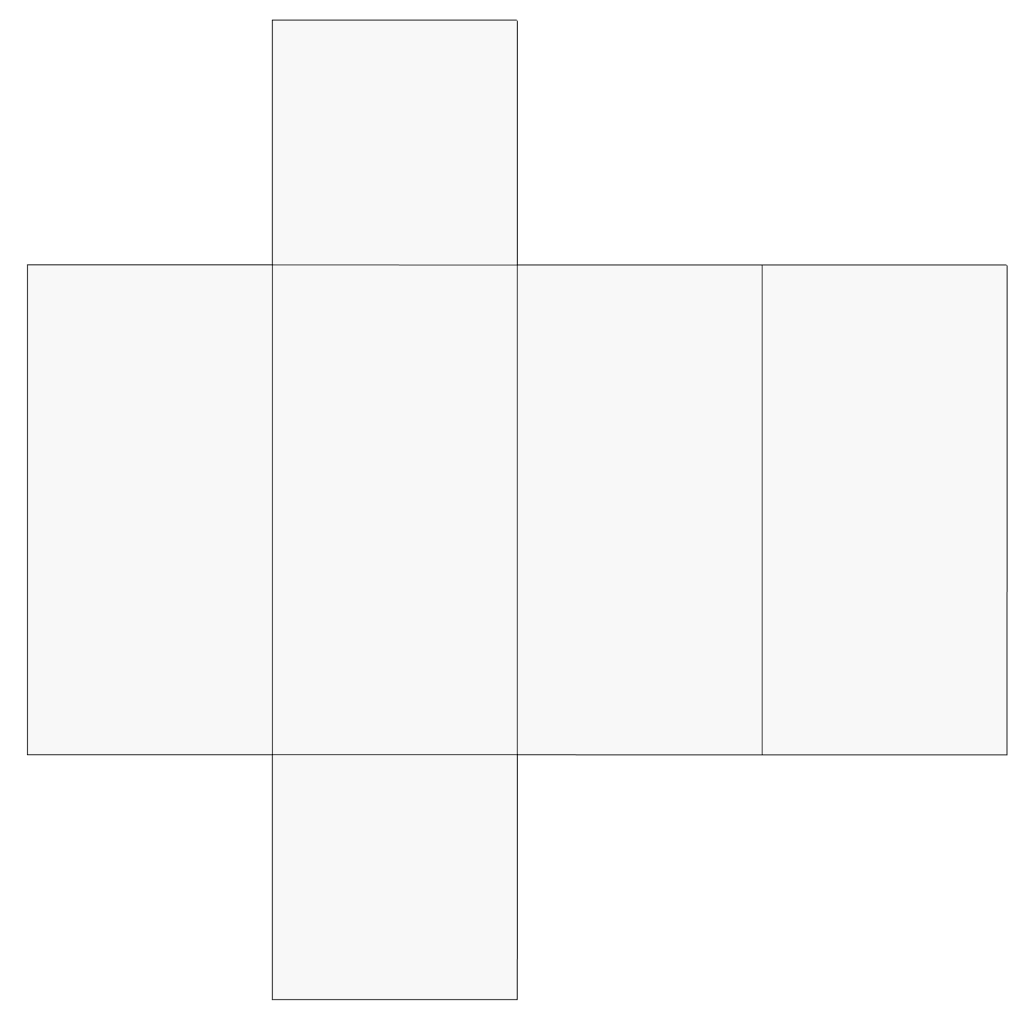
\includegraphics[scale=0.3]{mur_patron.png}
\caption{Patron du mur}
\end{center}
\end{figure}

Voici une des textures utilisée :
\begin{figure}[h]
\begin{center}
\includegraphics[scale=0.35]{mur_brique.png}
\caption{Texture d'un mur}
\end{center}
\end{figure}

\newpage
\subsubsection{Et après ?}
\par
Pour notre troisième soutenance je vais me fixer quelques objectifs à atteindre :
\newline

\par
\underline{Le multijoueur}
\newline
\par
Je compte terminer le multijoueur car même si aujourd'hui il est fonctionnel, je compte l'améliorer. Cela me permettra de progresser dans le code aussi.
\newline

\par
\underline{Les sons}
\newline
\par
Je compte rajouter des sons pour que l'ambiance du jeu soit complète lors de la troisième soutenance avec l’aide d’Anatole.
\newline

\par
\underline{L'éditeur de map}
\newline
\par
Enfin, je compte participer à l'édition des maps pour donner une dimension à notre jeu.
\newline

\par
\underline{Remerciements}
\newline
\par
Comment ne pas terminer encore une fois sur des remerciements à mon groupe qui reste soudé malgré nos différents? C'est donc pour cela que je remercie notre leader Louis qui soude quotidiennement notre équipe et nous encourage lorsque certains problèmes sont rencontrés, notre visionnaire Anatole qui aide à la projection du projet ainsi qu'à son aboutissement et toujours Khalis qui amène la bonne humeur tous les jours.

\newpage

\subsection {Anatole\textcolor {pseudoblue} {\textit {"Totonut"}} Moreau}

\subsubsection {Ce que j'ai réalisé}
\underline{Jeu.cs}
\par
Une grande partie de mon travail était déjà entamée grâce a la même structure qui se répète dans chaque classe de notre projet, c’est-à-dire l’existence d’une fonction Load, une fonction Update, et une fonction Draw. J’ai donc implémenté ces trois fonctions en utilisant des listes d’éléments déclarées comme attributs de la classe. Le jeu appelle à leurs tours les trois fonctions de chaque éléments de ces listes, et tout s’emboite correctement. Le rendu visuel a été visible grâce au travail graphique de Louis, Lenny et Khalis sur Blender et Photoshop. Toute la structure du code est ainsi visible dans ce fichier, qui est la base du déroulement du jeu. On y retrouve la boucle principale, qui gère les différents évènements du clavier. Tout ce qui concerne la camera a été fait par Louis. Les boutons actuellement gérés permettent de :
- Mettre le jeu en pause ;
- Quitter le jeu de force ;
- Déplacer le(s) joueur(s) ;
- Changer l’angle de vision du/des joueur(s) ;
- Monter/Descendre la camera, qui ne se déplace pas automatiquement avec le décors ;
- Arrêter /Reprendre la musique d’ambiance ;
Le jeu a également hérité d’une fonction chargerNiveau qui traite chaque information d’un fichier texte pour créer chaque élément de la carte un par un en les rajoutant aux listes initialisées au préalable.
\newline

\newpage
\underline{Editeur de map}

\begin{figure}[h]
\begin{center}
\includegraphics[scale=0.4]{editeur.png}
\caption{Editeur de map}
\end{center}
\end{figure}


\par
Lorsque le rendu d’affichage d’un sol et de murs était correct, il a fallu implémenter un rapide moyen de créer des niveaux pour la diversité du jeu. J’ai donc pris l’initiative de faire un petit éditeur de map, que l’on a rendu accessible aux utilisateurs pour rendre le jeu plus flexible en attendant sa finition. Il offre un terrain redimensionnable, et des éléments à y insérer. On y voit par exemple des points de spawn qui décident aleatoirement de la position d’apparition du joueur, des ennemis qui seront les éléments clés de la difficulté du niveau, des murs, caisses de munitions. Le tout doit être stocké dans un fichier texte placé dans le répertoire des ressources du jeu. Cet éditeur nous a permis de concevoir deux cartes qui s’apparentent à l’interieur d’une prison, mais tous les éléments ne s’affichent pas encore dans le rendu bien qu’ils soient traités par une fonction qui charge les éléments de la carte dans le jeu, car l’avancement graphique n’est pas terminé à cet instant. Ainsi, les munitions placées sur une carte n’afficheront rien. La sauvegarde s’effectue simplement a l’aide d’une énumeration d’éléments, chacun représenté par un int non signé, que l’on écrit sur le fichier texte, avant de le lire dans l’autre sens depuis Jeu.cs qui charge le niveau.
\newline
\newpage

\underline{Mode multijoueur}

\begin{figure}[h]
\begin{center}
\includegraphics[scale=0.4]{multi.png}
\caption{Mode multijoueur}
\end{center}
\end{figure}

\par
Khalis et moi avons fait la connaissance des viewports a l’occasion de l’implémentation d’un mode multijoueur. Bien que les objectifs ne soient pas encore disponible, le partage d’ecran est fini, avec l’acquisition de connaissances concernant les viewports. On a rencontre des difficultés au niveau du plein écran et de la barre de séparation, avant de constater que cela venait d’une mauvaise compréhension des viewports. Ce fut donc l’essentiel de notre tache. On a rencontré pas mal de problèmes pour le passage en plein écran, notamment pour l’affichage du hud (les vies, la barre de séparation) et on a remanié la surcharge de la fonction draw pour parvenir à nos fins.
\newline
\underline{Site web}
Le site web a subi une amélioration nette de la clarté du code, accompagné d’un changement esthétique. Avec Khalis à l’appui, le travail a été plus structuré et on a pu gagner en flexibilité. On a déplacé la barre de menu en haut de la page et on a dessiné un pied de page. Les divisions qui étaient placées de manière désordonnée ne le sont plus, et chaque classe de html a sa propre utilisation.
\newpage

\subsubsection {Mes impressions personnelles}
\par
Le temps a encore une fois été notre pire ennemi. Nous avons mal organisé nos rencontres et nous avons peiné au niveau du temps. Louis a bien géré la 3D et nous a facilité le travail. L’apprentissage a encore été ma principale motivation, et je n’ai pas été déçu : j’ai appris à structurer mon code, j’ai vu avec Khalis comment utiliser des viewports et des cameras distinctes. Il a été difficile de rendre « propre » le code qui s’occupe de l’affichage en multijoueur. Je pense que nous sommes en mesure d’améliorer hautement le jeu qu’on présente pour le moment car le niveau de mes camarades et moi-même a beaucoup évolué, et ayant travaillé avec Khalis à plusieurs reprises pour des petites tâches, je sais aujourd’hui qu’il est devenu plus confiant et performant, c’est très positif.
\newline

\subsubsection{Ce que je prévois}
La toisième soutenance va être riche en graphismes. Ainsi je prévois de lire le tutoriel d’Open Classrooms sur Blender pour aider Louis à réaliser des animations et autres modèles. On va donner au jeu sa dimension d’infiltration en rendant les ennemis intelligents, en leur fournissant des armes et en intégrants des objectifs. Les niveaux vont aussi avoir en quelque sorte une «âme», c’est-à-dire un thème propre, des objectifs propres, et pour cela, une classe Niveau va être implémentée. Je compte m’occuper des niveaux et des objectifs. Le menu devra comporter des options, et je compte attaquer cette partie du travail également. Le réseau s’annonce difficile d’après les recherches de Lenny à ce propos. Je vais donc aller chercher des informations de ce côté et participer à sa création. Nous prévoyons de rendre le jeu plus accessible en permettant aux visiteurs du site de choisir la langue utilisée. Cela fait beaucoup de choses en peu de temps, mais aujourd’hui les choses ont changé, et nous n’avons plus le choix : il faut travailler !


\newpage





\section{Tableau d'avancement}

\begin{tabular}{|c|p{2cm}|p{2cm}|p{2cm}|}


\hline
& Première soutenance & Deuxième soutenance & Troisième soutenance\\ 
\hline

Codage décors & 70\% & 100\% & 100\%\\
\hline
Codage objets & 70\% & 100\% & 100\%\\
\hline
Codage personnages & 70\% & 90\% & 100\%\\
\hline

Graphismes 2D/3D & - & 60\% & 100\%\\
\hline

Site web & 70\% & 100\% & 100\%\\
\hline

Son & 20\% & 80\% & 100\%\\
\hline

Collisions & - & 50\% & 100\%\\
\hline

Affichage & 70\% & 100\% & 100\%\\
\hline

Boucle de jeu & - & 50\% & 100\%\\
\hline

Interaction entre éléments du jeu & 20\% & 70\% & 100\%\\
\hline

Menu & 50\% & 100\% & 100\%\\
\hline

Réseau & - & 100\% & 100\%\\
\hline

Multijoueur & - & 60\% & 100\%\\
\hline

\end{tabular}

\section{Conclusion}
\par
Pendant notre période de travail, nous avons pris de l’avance sur nos prévisions ce qui nous permet de bien perfectionner certains détails.
\par
En effet, de nombreuses idées furent ajoutées  et les tâches que nous nous étions données à respecter depuis la première soutenance ont été remplies. Nous souhaitons vous montrer les avancées que nous avons réalisées car nous n’en sommes pas peu fiers !
\par
Notre jeu nous satisfait pour le moment mais nous ne nous relâchons pas et nous espérons que la soutenance se déroule dans les meilleures conditions.

\newpage
\thispagestyle{empty}
\pagestyle{fancyplain} \chead{}\lhead{\textit{Les Professionnels}} \rhead{\emph{\textit{Evasion}}}
\listoffigures

\end{document}
